\chapter{Gestión y Planificación del proyecto}
En este capítulo se tratarán todas las cuestiones relacionadas con la gestión del proyecto: la metodología de desarrollo escogida, la gestión del alcance, tiempo, riesgos y costes.

Lo que se busca con ello es determinar claramente los objetivos a cumplir durante la realización, así como asegurar el buen avance del proyecto repartiendo de forma adecuada los recursos, previniendo posibles problemas y estableciendo un marco de trabajo para estructurar, planificar y controlar el desarrollo del software.

\section{Gestión del alcance}
En esta sección se determinará el alcance general del proyecto, así como los criterios que serán necesarios para la aceptación de éste, y las restricciones a las que está sometido. Por último, se detallarán los entregables que se generarán al finalizar.

\subsection{Descripción del alcance del proyecto}
Para la creación de acertijos por parte de los usuarios y la posibilidad de que la comunidad de usuarios de la aplicación disponga de la posibilidad de poder resolver éstos e interactuar, es necesario tener en cuenta una serie de factores:

\begin{itemize}
    \item \textbf{Por parte de los usuarios:}
    \begin{itemize}
        \item \textbf{Datos personales del usuario:} será necesario almacenar datos personales tales como nombre y apellidos, contraseña y \textit{nick} o nombre de usuario.
        \item \textbf{Acertijos escritos:} es muy importante asociar cada usuario con el acertijo que él mismo ha escrito.
        \item \textbf{Propuestas de solución a acertijos:} también muy importante el registro en el sistema de las posibles propuestas de un usuario para la solución de los acertijos.
        \item \textbf{Valoración de las propuestas de solución a los acertijos del usuario:} un usuario podrá acceder a las soluciones propuestas para sus acertijos y puntuar según lo cerca que se encuentren de la solución final.
    \end{itemize}
    \item \textbf{Por parte de los acertijos:}
    \begin{itemize}
        \item \textbf{Datos específicos de cada acertijo:} será necesario almacenar el título, el acertijo, la solución al mismo, 3 pistas para facilitar el comienzo a los otros usuarios la búsqueda de la solución y el estado del porcentaje de resolución de la misma.
        \item \textbf{Acertijos escritos:} es muy importante asociar cada acertijo con el usuario que lo ha escrito.
        \item \textbf{Soluciones propuestas de cada acertijo:} también muy importante el registro en el sistema de las propuestas para la solución de cada acertijo.
    \end{itemize}
\end{itemize}

La aplicación contendrá dos funcionalidades principales, destacadas y que sustentarán el objetivo principal del proyecto: escritura de acertijos y resolución de los mismos.

Para la funcionalidad de escritura, el sistema será el encargado de almacenar los acertijos propuestos y mostrarlos al mundo. En la segunda funcionalidad nombrada, será el propio sistema el encargado de gestionar la interacción entre usuarios con el objetivo de resolver los enigmas.

\subsection{Criterios de aceptación}
El proyecto será aceptado si la aplicación será capaz de permitir a un usuario la escritura de un acertijo completo. Además, se podrá permitir al usuario proponer soluciones a distintos acertijos propuestos por otros usuarios. 

Por último, un usuario será capaz de poder evaluar las propuestas de solución de cada uno de sus acertijos y, éstos, automáticamente actualizarán su estado de resolución basándose en las puntuaciones de las mismas.
\subsection{Restricciones del proyecto}
El proyecto debe suponer un total de 12 créditos, es decir, unas 300 horas de trabajo, y debe ser entregado no más tarde del 07/09/2018.

\subsection{Entregables del proyecto}
Como resultado del proyecto se considerarán los siguientes entregables:
\begin{itemize}
    \item Código fuente de todo el software desarrollado.
    \item Memoria del trabajo de fin de grado.
\end{itemize}

\section{Metodología de desarrollo}
Antes de iniciar cualquier proyecto de desarrollo de software, es muy importante determinar y definir qué metodología se seguirá. El objetivo es establecer un plan de acción, reduciendo así el riesgo de que se sufran retrasos en el desarrollo, sobre costes, o un mal planteamiento que suponga el fracaso del proyecto en su totalidad. Probablemente en la práctica existan tantas metodologías de trabajo como proyectos de desarrollo, pero en todos los casos es necesario tener en cuenta las características y particularidades del proyecto a la hora de elegir y adaptar una metodología concreta al caso específico.

En el caso concreto de este proyecto, nos encontramos con varios factores importantes que resultan determinantes para la elección de una metodología concreta:

\begin{itemize}
    \item Al tratarse de una aplicación que necesita de interfaz, es necesario dedicar tiempo al desarrollo de la misma de una manera independiente a las demás partes. 
    \item En esta aplicación será necesaria la creación de una base de datos donde almacenar todos los acertijos, usuarios y propuestas de solución.
    \item Al tener que desarrollar una \textit{API Rest} que gestione las peticiones desde nuestra interfaz y nuestra base de datos, será necesario dedicar tiempo para el desarrollo de la misma, no de manera independiente, pues se necesita previamente una conexión de ésta con la base de datos.
\end{itemize}

Por ello, como metodología de desarrollo para mi proyecto lo mejor es crear una mezcla entre la metodología/framework  y la filosofía/práctiva \textit{DevOps}.

El lado \textit{Scrum} me aporta la creación de un marco de desarrollo de software con el que obtengo un mayor control y flexibilidad a la hora de enfrentar la incertidumbre, los cambios y los riesgos. Este marco permite realizar modificaciones a la planificación y requisitos de forma controlada y rápida, evitando así que el proyecto fracase por no realizarlos a tiempo. Además, permite que el contacto con el cliente sea mayor y continuo, evitando así que exista demasiada incertidumbre.

Con la cultura \textit{DevOps} se me proporciona la idea del desarrollo basado en pruebas \cite{desarrollotests}\cite{desarrollotests2}. Con esto obtengo que para cada entregable existe la garantía de que es un producto de calidad, pues ha pasado previamente todos los tests que describían su funcionalidad.

\subsection{Scrum}

Las metodologías ágiles surgen como respuesta a los problemas característicos de las metodologías tradicionales. Tanto Scrum como otras metodologías ágiles (Iconix, Cristal Methods), se basan en los siguientes principios:

\begin{itemize}
    \item Es más importante que se desarrolle un producto de software de calidad y que funcione que escribir una documentación exhaustiva. 
    \item Las interacciones entre individuos son más importantes que las herramientas y procesos utilizados.
    \item La comunicación con el cliente es vital para el éxito del proyecto.
    \item Aún cuando establecer un plan es necesario, es más importante el contar con una buena capacidad de respuesta ante los cambios.
\end{itemize}

\subsubsection{Características de Scrum}
Esta metodología se centra en el desarrollo incremental iterativo. A cada una de estas iteraciones las llamaremos \textbf{Sprints}, y normalmente serán de una duración corta entre 3 y 4 semanas. Cada Sprint termina con una pieza clave de software completa y funcional.

Se prioriza el trabajo que resulta más valioso para el desarrollo del proyecto, con el objetivo de maximizar la utilidad de lo que se desarrolla. Los requisitos y la prioridad de éstos se revisan regularmente, normalmente al inicio de cada Sprint. El objetivo es construir de forma incremental un producto que se ajuste realmente a las necesidades del cliente, asegurando así su satisfacción.

Para mantener el ritmo de trabajo, sometido a constantes cambios, es necesario que el equipo se centre en construir \textbf{software de calidad}, pero para que esto pueda ser posible son necesarios dos aspectos: la gestión del proyecto debe asegurar una buena definición de las características deseables y evitar cualquier obstáculo que pueda afectar el trabajo del equipo; además el cliente debe entusiasmarse realmente por el proyecto desarrollado, de forma que exista un compromiso real que se mantenga tras la finalización de cada sprint con el objetivo de mantener la comunicación constantemente y conocer así sus necesidades reales.

\subsubsection{Herramientas y roles}
Sprint define todas las funcionalidades requeridas del producto a desarrollar en el \textit{Product Backlog}, determinando su prioridad, valor y riesgo, además de una estimación (de forma muy general) de la cantidad de trabajo que supone desarrollarla. Esta lista evoluciona a lo largo de todo el desarrollo.
		
		Además esta metodología define tres roles: el \textit{Scrum master}, el \textit{Product owner} y el equipo de desarrollo.
			\begin{itemize}
				\item \textbf{\textit{Scrum Master}}: es el líder del equipo. Se encarga de asegurarse de que se está siguiendo la metodología, se cumplen sus valores y prácticas. 
				\item \textbf{\textit{Product Owner}}: es el encargado de gestionar el desarrollo y el intermediario entre el cliente y el equipo. Se encarga de organizar y priorizar todas las funcionalidades requeridas.
				\item \textbf{Equipo de desarrollo}: es la pieza clave del proyecto. Puede estar a su vez subdividido en equipos de desarrollo, testing y despliegue. 
			\end{itemize}
\subsubsection{Ciclo de trabajo}
	    Scrum define un evento principal llamado Sprint, el cual corresponde con una ventana de trabajo que, tras su finalización, produce una versión funcional del producto. Dentro de cada sprint tienen lugar una serie de eventos. La figura \ref{fig::cicloDeVidaSprint} muestra el ciclo de vida de un sprint. 
	    
\begin{figure}
    \centerline{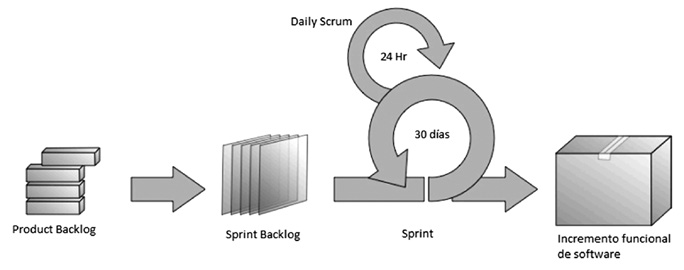
\includegraphics[width=11cm]{figuras/fasesDeUnSprint.png}}
    \caption{Ciclo de vida de un sprint}
    \label{fig::cicloDeVidaSprint}
\end{figure}

\begin{enumerate}
		\item \textbf{Planificación de la iteración (\textit{Sprint planning})}: se define el plan de trabajo de este Sprint especifico determinando qué se entregara y cómo se logrará. Es decir, se determinan las funcionalidades a implementar y la estimación de cantidad de trabajo. Con todo esto, y partiendo de la información en el \emph{Product backlog}, se establece el \emph{Sprint backlog}.
		\item \textbf{Reunión diaria (\textit{Daily meeting})}: cada día se realiza una reunión para explicar los objetivos que se han alcanzado desde la ultima reunión y determinar qué se realizará el día siguiente. Esto permite identificar problemas rápidamente y evitar que se retrase el ritmo de trabajo. \item \textbf{Revisión de la iteración (\emph{Sprint review})}: se realiza tras la finalización del Sprint completo. Se revisa todo lo que se hizo y lo que no, se comentan los problemas que tuvieron lugar y cómo se resolvieron, y se revisan los resultados obtenidos. 
		\item \textbf{Retrospectiva de la iteración (\emph{Sprint retrospective})}: esta reunión tiene el objetivo de analizar los puntos a mejorar y los puntos fuertes del equipo con el fin de aumentar la productividad.
		\item \textbf{Replanificación}: conjuntamente con el cliente se revisa la planificación teniendo en cuenta los posibles cambios que hayan podido surgir durante el \emph{Sprint}.
\end{enumerate}
			
\subsection{Aplicación de Scrum a este proyecto}
Dado que la mayoría de las practicas de Scrum están centradas en mejorar la productividad de un equipo, se han realizado una serie de adaptaciones teniendo en cuenta las características y circunstancias del proyecto. Se ha prescindido de la reunión diaria, pues el equipo de desarrollo está formado por una única persona. En este caso los sprints tuvieron una duración de inicial de 3 semanas, por lo que en lugar del \textit{Daily meeting} se ha optado por realizar una reunión semanal en la que se comentaba todo lo realizado hasta el momento y todas las actividades pendientes de abordar. Además, la reunión al final de cada sprint se realizó, en su mayoría, únicamente con los tutores y no con el cliente. Sin embargo, se mantuvo comunicación con este constantemente a lo largo de todo el desarrollo.

\subsection{DevOps}

Las antiguas metodologías de desarrollo de software separaban en dos sectores bien diferenciados aquellos que escribían el software (Dpto. Desarrollo) de aquellos que desplegaban en la nube (Dpto. Sistemas) \cite{devops5}.

DevOps surge con la idea de romper esta división y unir en un solo equipo a aquellos que desarrollan software y aquellos que lo despliegan. Esta unión proporciona transparencia a la hora de consultar el estado del producto y las distintas etapas que ha superado o superará.

La filosofía DevOps se basa en los mismos principios que las metodologías ágiles. Sin embargo, con DevOps se quiere fomentar una cultura de equipo, en la que todas las personas que formen el equipo sepan qué está haciendo cada una.

\subsubsection{Características de DevOps}
Esta filosofía busca la calidad de un producto software, creado por un equipo que se adapte rápido a los cambios e inconvenientes que aparezcan a lo largo de su desarrollo. Estos cambios deben ser identificados con rapidez para su posterior solución.

DevOps engloba todas las buenas prácticas a tener en cuenta a la hora de la entrega, el desarrollo y la administración de aplicaciones a lo largo del ciclo de vida de desarrollo de software: \cite{devops7}

\begin{itemize}
    \item Desarrollo y revisión de código con la ayuda de un controlador de versiones.
    \item Uso de herramientas de integración continua
    \item Continuo testeo del producto para obtener un software de calidad
    \item Uso de un gestor de repositorio optimizar la descarga y el almacenamiento de archivos binarios utilizados y producidos en el desarrollo de software.
    \item Uso de un gestor que automatice el proceso de despliegue
    \item Uso de un gestor de aprovisionamiento que nos cargue las configuraciones que necesarias de nuestro proyecto
    \item Monitorización del rendimiento de la aplicación
\end{itemize}

\subsection{Aplicación de DevOps a este proyecto}

Para este proyecto se usará Git \footnote{https://git-scm.com/} como herramienta para el control de versiones y GitHub \footnote{https://github.com/} como servicio público donde almacenar el repositorio de la aplicación.

Es fundamental en este proyecto el desarrollo basado en pruebas y la integración continua en el respositorio. El código debe de estar testeado previamente antes de añadirlo oficialmente al repositorio del mismo si se quiere obtener un software de calidad.

En este proyeco el equipo está formado por una persona, por lo que el mismo equipo será transparente y formado por el sector de desarrollo y el sector de despliegue.


\subsection{Combinación de Scrum y DevOps}

Como se ha explicado anteriormente, Scrum nos define un marco para el desarrollo de la aplicación. Un marco donde se definen Sprints para la consecución de objetivos.

Scrum se usará en este proyecto como una estructura que ayude a 

Dentro de cada Sprint, DevOps ayudará a la obtención de esos objetivos gracias a su filosofía, sobre todo su buena práctica relacionada en el desarrollo basado en pruebas, herramientas de automatización para el despliegue y la revisión del código gracias a un controlador de versiones.

\section{Gestión de la configuración}
En esta sección se define la gestión de la configuración bajo la cual desarrollaremos todas las actividades que impliquen la creación, modificación o eliminación de alguno de los elementos de trabajo que conforman este proyecto, asegurando así que todo lo que concierne al proyecto sea válido durante la vida del mismo.

 Teniendo en cuenta que los elementos de trabajo de este proyecto son los ficheros de código fuente y todos los archivos que conforman la documentación, abordaremos esta sección especificando, de forma independiente, cómo se ha tratado cada tipo de elemento de trabajo.
 
\subsection{Gestión del código}

Para la gestión del código se creará un repositorio local con un  sistema de control de versiones, que a su vez se sincronizará con un repositorio remoto en \textit{GitHub}, y por lo tanto almacenado en la nube. \textit{GitHub} es un servicio web de control de versiones y desarrollo de software basado en \textit{Git}, publicado bajo una Licencia de código abierto. Esta copia remota previene el riesgo de pérdida del código fuente.

\subsection{Gestión de la documentación}
Para almacenar la documentación de este proyecto se utilizará un repositorio en \textit{GitHub} llamado \textbf{Memoria\_TFG\_GuillermoMuriel} \footnote{https://github.com/guillesiesta/Memoria\_TFG\_GuillermoMuriel}.

Esta plataforma permite la creación de un repositorio cuyo lenguaje principal será LateX, y le añade una licencia de código abierto.

En cuanto a la edición y gestión de la memoria del proyecto, se utilizará la plataforma online \textit{Overleaf v2}\footnote{https://v2.overleaf.com/}. Dispone de control de versiones y edición en concurrencia. De la misma forma, al estar almacenada en la nube, se previene el riesgo de pérdida.

\section{Gestión del tiempo}
En este apartado se trata la planificación temporal del proyecto y las fases de la misma. Si bien se ha  establecido una planificación inicial, las tareas a realizar se especificarán de forma concreta a medida que se avance en el desarrollo del proyecto en función de los resultados obtenidos tras la finalización de cada sprint.

\subsection{Planificación inicial}
\subsection{Planificación final}


\section{Gestión de riesgos}
\subsection{Identificación de riesgos}
\subsection{Análisis de riesgos}
\subsection{Planificación de la respuesta a los riesgos}
\subsection{Riesgos materializados}

\section{Gestión de costes}
\subsection{Costes de recursos humanos}
\subsection{Costes de material}
\subsection{Costes de indirectos}
\subsection{Costes total del proyecto}

